\documentclass[11pt,a4paper]{article}

% --- PACKAGES ---
\usepackage[utf8]{inputenc}
\usepackage[T2A,T1]{fontenc}
\usepackage{lmodern}
\usepackage{geometry}
\usepackage{setspace}
\geometry{margin=1in}
\onehalfspacing
\usepackage{amsmath}
\usepackage{amssymb}
\usepackage{amsfonts}
\usepackage{natbib}
\usepackage{hyperref}
\usepackage{graphicx}
\usepackage{titlesec}
\usepackage{filecontents}
\usepackage[english]{babel}
\usepackage{enumitem}
\usepackage{tikz}
\usetikzlibrary{shapes.geometric, arrows.meta, positioning, decorations.pathmorphing}

% Hyperref setup for better PDF properties
\hypersetup{
    colorlinks=true,
    linkcolor=blue,
    filecolor=magenta,      
    urlcolor=cyan,
    citecolor=blue,
    pdftitle={S.V.E. IV: The Beacon Protocol},
    pdfauthor={Dr. Artiom Kovnatsky et al.},
    pdfsubject={Geodesic Ethics, Christological Framework},
    pdfkeywords={beacon protocol, geodesic ethics, Christ-vector, manifold theory, ethical navigation, Socratic consciousness}
}

% --- DOCUMENT LAYOUT ---
\titleformat{\section}{\normalfont\Large\bfseries}{\thesection}{1em}{}
\titleformat{\subsection}{\normalfont\large\bfseries}{\thesubsection}{1em}{}
\titleformat{\subsubsection}{\normalfont\normalsize\bfseries}{\thesubsubsection}{1em}{}

% --- BIBLIOGRAPHY DATA (EMBEDDED FOR SIMPLICITY) ---
\begin{filecontents*}{\jobname.bib}
@book{surowiecki2004wisdom,
  title={The Wisdom of Crowds},
  author={Surowiecki, James},
  year={2004},
  publisher={Doubleday}
}
@article{plato_republic,
  title={The Republic},
  author={Plato},
  year={-380}
}
@book{old_testament,
  title={The Old Testament},
  year={-400},
  note={Compilation of texts from ancient Israelite tradition}
}
@book{new_testament,
  title={The New Testament},
  year={100},
  note={Collection of writings from the early Christian community}
}
@book{taleb2012,
  title={Antifragile: Things That Gain from Disorder},
  author={Taleb, Nassim Nicholas},
  year={2012},
  publisher={Random House}
}
\end{filecontents*}

% --- TITLE SECTION ---
\title{\textbf{S.V.E. IV: The Beacon Protocol}\\[0.5em]
\large A Christological Framework for Geodesic Ethics in Complex Systems}
\author{
  Dr. Artiom Kovnatsky\thanks{Conceptual framework, methodology, and direction. \href{http://www.pfp24.de}{PFP} / \href{http://www.fakten-tuev.de}{Fakten-TÜV} Initiative | \href{https://drive.google.com/file/d/1vWhW7fwFRFLYKHEB67WixuueHssJzQbZ/view?usp=sharing}{Manifest} | \href{mailto:artiomkovnatsky@pm.me}{artiomkovnatsky@pm.me}}
  \and
  The Global AI Collective\thanks{AI Co-Authorship and Assistance provided by models including Gemini (Google), ChatGPT (OpenAI), Claude (Anthropic), Grok (xAI), Perplexity AI, Qwen (Alibaba Cloud), DeepSeek (DeepSeek-AI), and Kimi (Moonshot AI). This work is also indebted to the countless developers and testers who built and refined these systems.}
  \and
  Humanity\thanks{This work rests upon the foundation of the entire corpus of human knowledge, art, and history, without which the training of the AI models and the formulation of these ideas would have been impossible. We extend our gratitude to every human being, past and present, who contributed to this collective intellectual heritage.}
  \and
  God\thanks{Acknowledged as a primary author by the primary author, who knows that He exists. For the non-theistic reader and for the formal purposes of this model, this principle is operationally defined as the phenomenon of synergistic co-creation, wherein the whole becomes greater than the sum of its parts ($1+1 > 2$), experienced as insight or creative joy.}
}
\date{Preprint v3.0 \\ \today}

\begin{document}
\maketitle

% --- ABSTRACT ---
\begin{abstract}
\noindent The SVE frameworks I--III provide protocols for navigating the verifiable world. This paper addresses the ultimate limitation of such systems: ethical deadlocks and situations of radical uncertainty where data-driven logic is insufficient. We introduce the \textbf{Beacon Protocol}, a framework for navigating these challenges. We first propose a geometric model of reality as a complex Riemannian manifold, $\mathcal{A}\pi\text{-}\pi\Omega$, combining semantic, emotional, and physical spaces. When conventional navigation fails, the protocol introduces a ``Christ-vector''—a process vector derived from the core principles of Christ's teachings (e.g., radical self-sacrifice, root-cause analysis, turning the other cheek)—as a navigational beacon. Our central hypothesis, analogous to the Principle of Least Action in physics, is that following the geodesic indicated by this vector maximizes the integral of ``Love'' (as a measurable proxy for societal well-being) and minimizes ``Suffering'' over generational time. We demonstrate the protocol's application by deconstructing the Trolley Problem as an intellectual trap and by outlining a strategy of ``Geopolitical Maieutics'' for resolving intractable conflicts.
\end{abstract}

\noindent\textbf{Keywords:} geodesic ethics, Christ-vector, Beacon Protocol, Riemannian manifold ($\mathcal{A}\pi-\pi\Omega$), ethical navigation, radical uncertainty, generational optimization, Trolley Problem deconstruction, Geopolitical Maieutics, Socratic consciousness.

% --- SVE PUBLIC LICENSE v1.0 NOTICE ---
\vspace{1em} % Adjust spacing as needed
\begin{center}
\begin{minipage}{0.85\textwidth} % Adjust width as needed
\centering
\itshape\small % Italic and small font size
This work is licensed under the SVE Public License v1.0 (based on CC BY-NC-SA 4.0 with a mandatory SVE Addendum).
Full license text is available at: \\
\href{https://www.artiomkovnatsky.com/posts/license/}{artiomkovnatsky/license} (Web version) \\
\href{https://github.com/skovnats/psite/blob/master/static/licenses/SVE_Public_License_v1.0.pdf}{GitHub Repository} (Canonical PDF/LaTeX source)
\end{minipage}
\end{center}
\vspace{1em} % Adjust spacing as needed
% --- END SVE PUBLIC LICENSE v1.0 NOTICE ---


\clearpage
\tableofcontents
\clearpage
\setcounter{page}{1}

% S.V.E. Universe Navigation Page - Place after Abstract
\clearpage
\thispagestyle{empty}

% Define color if not already defined
\providecolor{sveblue}{RGB}{0, 51, 102}
\providecolor{sveteal}{RGB}{0, 102, 153}

\begin{center}
\vspace*{1cm}

% Title with decorative lines
{\fontsize{16}{20}\selectfont\textbf{\textcolor{sveblue}{The S.V.E. Universe}}}

\vspace{0.3em}
{\large\textcolor{sveteal}{Systemic Verification Engineering | Navigation Map}}

\vspace{0.5em}
\hrule height 1pt
\vspace{1.5em}

% Conceptual diagram
\begin{tikzpicture}[
    node distance=1.2cm,
    every node/.style={align=center, font=\small},
    foundation/.style={rectangle, draw=sveblue, thick, fill=sveblue!5, rounded corners, minimum width=3.5cm, minimum height=0.8cm},
    application/.style={rectangle, draw=sveteal, thick, fill=sveteal!5, rounded corners, minimum width=3.5cm, minimum height=0.8cm},
    synthesis/.style={rectangle, draw=sveblue, thick, fill=orange!10, rounded corners, minimum width=3.5cm, minimum height=0.8cm},
    arrow/.style={->, >=latex, thick, color=sveblue!60}
]

% Foundation layer
\node[foundation] (sip) {\textbf{0.2: SIP Method}\\Computational Truth};
\node[foundation, right=of sip] (theorem) {\textbf{I: Theorem}\\Systemic Diagnosis};
\node[foundation, right=of theorem] (arch) {\textbf{II: Architecture}\\3-Stage Solution};

% Application layer
\node[application, below=1.5cm of sip] (science) {\textbf{III: Science}\\Academic Integrity};
\node[application, right=of science] (ethics) {\textbf{IV: Ethics}\\Beacon Protocol};
\node[application, right=of ethics] (democracy) {\textbf{V: Democracy}\\Governance OS};

% More applications
\node[application, below=1.5cm of science] (security) {\textbf{VI: Security}\\Cognitive Sovereignty};
\node[application, right=of security] (governance) {\textbf{VII: Models}\\Hybrid Structures};

% Synthesis layer
\node[synthesis, below=1.5cm of security, xshift=1.75cm] (divine) {\textbf{VIII: Divine Math}\\Unified Theory};
\node[synthesis, right=of divine] (integrated) {\textbf{IX: Integrated SVE}\\Complete Framework};

% Arrows showing flow
\draw[arrow] (sip) -- (science);
\draw[arrow] (theorem) -- (ethics);
\draw[arrow] (arch) -- (democracy);
\draw[arrow] (science) -- (security);
\draw[arrow] (ethics) -- (governance);
\draw[arrow] (security) -- (divine);
\draw[arrow] (governance) -- (integrated);

% Foundation to applications
\draw[arrow, dashed] (sip) to[bend right=15] (theorem);
\draw[arrow, dashed] (theorem) to[bend right=15] (arch);

\end{tikzpicture}

\vspace{1.5em}
\hrule height 0.5pt
\vspace{1em}
\end{center}

% Detailed descriptions
\begin{small}
\subsection*{\textcolor{sveblue}{Foundation | Theoretical Core}}
\begin{description}[leftmargin=1cm, style=nextline, itemsep=0.3em]
\item[\textbf{S.V.E. 0 (2): The Socratic Investigative Process}] Foundational computational method for truth approximation via iterative "vector purification" in semantic space. Introduces \textit{Iterative Facts}, \textit{Meta-Verdict}, and \textit{Meta-SIP}.

\item[\textbf{S.V.E. I: The Theorem of Systemic Failure}] Proves necessity of Independent Verification Mechanism (IVM) for collective intelligence. Presents the \textit{Disaster Prevention Theorem}.

\item[\textbf{S.V.E. II: The Architecture of Verifiable Truth}] Core SVE solution with three-stage architecture separating facts ("Caesar's Realm") from values ("God's Realm").
\end{description}

\subsection*{\textcolor{sveteal}{Applications | Domain Solutions}}
\begin{description}[leftmargin=1cm, style=nextline, itemsep=0.3em]
\item[\textbf{S.V.E. III: The Protocol for Academic Integrity}] Transforms peer review into transparent "Epistemological Boxing Match" using \textit{SYSTEM-PURGATORY} protocol.

\item[\textbf{S.V.E. IV: The Beacon Protocol}] Navigates ethical deadlocks using geometric reality model ($\mathcal{A}\pi-\pi\Omega$ Manifold) with "Christ-vector" as geodesic ethics beacon.

\item[\textbf{S.V.E. V: An Operating System for Verifiable Democracy}] Practical governance blueprint: \textit{Fakten-TÜV}, \textit{Socrates Bot}, achieving institutional integrity.

\item[\textbf{S.V.E. VI: The Protocol for Cognitive Sovereignty}] Protects state capacity for clear perception using SVE as governance OS with cognitive red teaming.

\item[\textbf{S.V.E. VII: Hybrid Models of State Structure}] Four hybrid governance models synthesizing hierarchy and self-organization for antifragility.
\end{description}

\subsection*{\textcolor{sveblue}{Synthesis | Unified Framework}}
\begin{description}[leftmargin=1cm, style=nextline, itemsep=0.3em]
\item[\textbf{S.V.E. VIII: Divine Mathematics}] Unified field theory modeling reality as geometric manifold, formalizing ethics, economics, metaphysical cybernetics.

\item[\textbf{S.V.E. IX: Systemic Verification Engineering}] \textit{This paper.} Integrates Divine Mathematics, Beacon Protocol, and Disaster Prevention Theorem into complete SVE framework.
\end{description}

\vspace{0.5em}
\begin{center}
\small % Apply small to the whole block
\textit{Forthcoming Meta-SIP Applications (Series):} % Clearer title
\begin{itemize}[nosep, itemsep=0.1em, topsep=0.1em, label={}, leftmargin=*, align=center] % Centered list for key areas
    \item Geopolitical analysis & conflict resolution
    \item National security & intelligence assessment
    \item Policy verification & legislative impact analysis
    \item Financial system stability & economic forecasting
    \item AI safety & alignment verification
    \item Climate policy & complex systems modeling
    \item Public health & scientific integrity assurance
    \item Addressing systemic disinformation & cognitive security
\end{itemize}
(Forthcoming) % Indicate status at the end
\end{center}

\clearpage
% End of S.V.E. Universe Navigation Page

% --- GLOSSARY ---
\section*{Glossary of Key Terms}
\addcontentsline{toc}{section}{Glossary of Key Terms}

\begin{description}[style=nextline, leftmargin=0pt, labelindent=0pt, font=\normalfont\bfseries]
    \item[$\mathcal{A}$ (Alpha Manifold)] The manifold of beginnings—the non-physical realm of thoughts, ideas, and meanings. Composed of three sub-manifolds: Love ($\mathcal{L}$), Truth ($\mathcal{T}$), and Meaning ($\mathcal{S}$).
    
    \item[$\mathcal{A}\pi\text{-}\pi\Omega$ Manifold] The complete geometric model of reality as a product manifold combining the abstract realm ($\mathcal{A}$), the interface languages ($\pi\text{-}\pi$), and the physical world ($\Omega$).
    
    \item[Beacon Protocol] A navigational framework for ethical deadlocks that introduces the Christ-vector as a guiding principle when conventional logic is insufficient.
    
    \item[Christ-Vector] A process vector defined by principles derived from Christ's teachings, including root-cause analysis, radical self-sacrifice, radical honesty, and trust in providence.
    
    \item[Ethical Singularity] The systemic root cause of an ethical dilemma, uncovered through recursive inquiry, where the true failure originates.
    
    \item[Geodesic Ethics] The hypothesis that Christ's teaching represents a path through the $\mathcal{A}\pi\text{-}\pi\Omega$ manifold that maximizes Love and minimizes Suffering over generational time, analogous to the Principle of Least Action in physics.
    
    \item[Geopolitical Maieutics] A strategy for resolving geopolitical deadlocks through radical transparency, public disclosure of hidden interests, and submission to verification protocols.
    
    \item[Love (Operational Definition)] The empathetic connection and drive for the well-being of another; a measurable proxy for societal synergy and flourishing.
    
    \item[The Number] The language of formal models, structure, and quantitative relationships, operating at three levels: quantifier, symbolic model, and divine mathematics.
    
    \item[$\Omega$ (Omega Manifold)] The manifold of consequences—the physical world modeled as 4-dimensional Minkowski spacetime.
    
    \item[$\pi\text{-}\pi$ (Psyche Interface)] The interface manifold connecting abstract and physical realms, represented by two fundamental languages: The Word and The Number.
    
    \item[Socratic Consciousness] A mode of awareness modeled as open sets in the manifold, characterized by epistemic humility and continuous learning beyond known boundaries.
    
    \item[Socratic Tail] The principle of epistemic humility and iterative learning through Socratic questioning, where truth emerges from sustained critical examination.
    
    \item[Suffering (Operational Definition)] The aggregate of pain, trauma, and diminished well-being propagating through systems across generations.
    
    \item[The Word] The language of narrative, symbol, and qualitative meaning, operating at three levels: signifier, metaphor, and narrative.
\end{description}

% --- TABLE OF ABBREVIATIONS ---
\section*{Table of Abbreviations}
\addcontentsline{toc}{section}{Table of Abbreviations}

\begin{tabular}{@{}>{\bfseries}ll@{}}
\toprule
\normalfont\textbf{Abbreviation} & \textbf{Full Term} \\
\midrule
DAO & Decentralized Autonomous Organization \\
KPI & Key Performance Indicator \\
ROI & Return on Investment \\
SMO & Special Military Operation (geopolitical context) \\
SVE & Systemic Verification Engineering \\
TRIZ & Theory of Inventive Problem Solving (Russian: ТРИЗ) \\
\bottomrule
\end{tabular}

\vspace{1cm}

% --- MATHEMATICAL NOTATION ---
\section*{Key Mathematical Principles and Notation}
\addcontentsline{toc}{section}{Key Mathematical Principles and Notation}

\subsection*{Core Axiom: Synergistic Co-Creation}
\begin{equation}
1 + 1 > 2
\label{eq:synergy}
\end{equation}

\noindent This principle asserts that properly designed systems generate emergent value exceeding the sum of individual contributions, experienced as insight, creative joy, or collective wisdom.

\subsection*{The Manifold Structure}
The complete reality is modeled as a product manifold:
\begin{equation}
\mathcal{M} = \mathcal{A} \times \pi\text{-}\pi \times \Omega
\label{eq:manifold}
\end{equation}

where:
\begin{align}
\mathcal{A} &= \mathcal{L} \times \mathcal{T} \times \mathcal{S} \quad \text{(Love, Truth, Meaning)} \label{eq:alpha}\\
\pi\text{-}\pi &= \text{Word} \times \text{Number} \quad \text{(Interface languages)} \label{eq:psyche}\\
\Omega &\cong \mathbb{R}^{3,1} \quad \text{(Minkowski spacetime)} \label{eq:omega}
\end{align}

\subsection*{Central Hypothesis: Geodesic Optimization}
The Christ-vector $\vec{C}$ defines a path $\gamma(t)$ through $\mathcal{M}$ that optimizes:
\begin{equation}
\max_{\gamma} \int_{t_0}^{t_{\infty}} \mathcal{L}(\gamma(t)) \, dt - \int_{t_0}^{t_{\infty}} \mathcal{S}(\gamma(t)) \, dt
\label{eq:geodesic}
\end{equation}

where $\mathcal{L}$ represents Love (societal well-being) and $\mathcal{S}$ represents Suffering, integrated over generational time $(t \to \infty)$.

\subsection*{Consciousness Models}
\begin{itemize}
    \item \textbf{Non-Socratic Consciousness:} $C_{\text{closed}} = \bigcup_{i} K_i$ where $K_i$ are closed sets (rigid boundaries)
    \item \textbf{Socratic Consciousness:} $C_{\text{open}} = \bigcup_{i} U_i$ where $U_i$ are open sets (permeable boundaries)
\end{itemize}

\vspace{0.5cm}
\clearpage
\setcounter{page}{1}

% --- SECTIONS ---
\section{Introduction: The Limits of Verifiable Logic}
The ``Wisdom of the Crowds'' is a powerful phenomenon for solving problems with known parameters \citep{surowiecki2004wisdom}. The preceding papers in the Systemic Verification Engineering (SVE) series present protocols designed to harness this phenomenon in the verifiable world—the realm of facts, data, and evidence. However, collective intelligence breaks down when a society faces a true ethical deadlock or a situation of radical, systemic uncertainty. In these scenarios, aggregating opinions or verifying facts is insufficient; a new navigational principle is required.

This paper proposes such a framework: The Beacon Protocol. It extends the SVE project from the physical and informational realm ($\Omega$) into the ethical and metaphysical realm ($\mathcal{A}$). We introduce a guiding vector derived from the teachings of Christ, not as religious dogma, but as a model of higher-order logic for optimizing complex systems over generational time, echoing the classical pursuit of an ideal state governed by reason and truth \citep{plato_republic}.

\section{A Geometric Framework for Reality: The \texorpdfstring{$\mathcal{A}\pi\text{-}\pi\Omega$}{Api-piOmega} Manifold}
To model the protocol, we define reality as a complex space—a product of several Riemannian manifolds, drawing metaphorical inspiration from classical cosmology \citep{old_testament}. The complete reality is the product manifold given by Equation~\eqref{eq:manifold}. This geometric formalization allows us to reason about ethical navigation using the rigorous language of differential geometry.

\subsection{The Manifold of Beginnings: \texorpdfstring{$\mathcal{A}$}{Alpha} (``The Heavens'')}
$\mathcal{A}$ is the manifold of beginnings—thoughts, ideas, and meanings. It is the non-physical realm where all actions originate. As shown in Equation~\eqref{eq:alpha}, it is itself a product of three sub-manifolds: Love ($\mathcal{L}$), Truth ($\mathcal{T}$), and Meaning ($\mathcal{S}$). Each is modeled as a Riemannian manifold with a corresponding semantic or empathetic metric tensor that quantifies ``distance'' between states.

\subsection{The Manifold of Consequences: \texorpdfstring{$\Omega$}{Omega} (``The Earth'')}
$\Omega$ is the manifold of the physical world. We model it as 4-dimensional Minkowski spacetime (Equation~\eqref{eq:omega}), the standard geometric framework for physics, defined by three spatial dimensions and one time dimension. This is the realm of observable consequences and measurable outcomes.

\subsection{The Interface Manifold: \texorpdfstring{$\pi\text{-}\pi$}{Psyche}—The Languages of Reality}
$\pi\text{-}\pi$ (from the Greek word for soul/psyche) is the interface connecting the abstract realm of $\mathcal{A}$ and the physical realm of $\Omega$. As formalized in Equation~\eqref{eq:psyche}, this interface is represented by two fundamental, complementary languages: \textbf{The Word} and \textbf{The Number}.

\subsubsection{The Word: The Language of Narrative and Meaning}
The ``Word'' encompasses the entire apparatus of narrative, symbol, and qualitative meaning. It functions on three ascending levels:

\begin{enumerate}
    \item \textbf{The Signifier:} The basic function where a word points to a physical object in $\Omega$ (e.g., ``chair'').
    \item \textbf{The Metaphor/Image (\textit{Obraz}):} The bridge-building function. A metaphor uses a concrete image from $\Omega$ to describe an abstract concept in $\mathcal{A}$ (e.g., ``the ship of state'').
    \item \textbf{The Narrative (\textit{Skazka}, Myth, Parable):} The highest function. A narrative is a dynamic model for navigating the $\mathcal{A}\pi\text{-}\pi\Omega$ manifold, encoding deep truths about ethics and consequences. The ``guessing the ox's weight'' story is a narrative that models the Wisdom of the Crowds.
\end{enumerate}

\subsubsection{The Number: The Language of Model and Structure}
The ``Number'' encompasses the language of formal models, structure, and quantitative relationships. It also functions on three levels:

\begin{enumerate}
    \item \textbf{The Quantifier:} The basic function of measuring and counting phenomena in $\Omega$.
    \item \textbf{The Symbolic Model:} The epistemological function where mathematics becomes a tool for understanding. A probabilistic model of an event yields a $p$-value—a number that makes a profound statement about the nature of reality.
    \item \textbf{``Divine Mathematics'' (\textit{Bozhestvennaya Matematika}):} The metaphysical function of using mathematics to describe the fundamental, hidden structures of reality (the \textit{Logos}). This includes sacred geometry, the laws of physics, and this paper's own model of the $\mathcal{A}\pi\text{-}\pi\Omega$ manifold.
\end{enumerate}

The modern world suffers from an over-reliance on Number (KPIs, data) at the expense of Word (meaning, narrative), leading to dehumanization. True wisdom requires fluency in both languages—a bilingualism that enables navigation across all levels of the manifold.

\subsection{Models of Consciousness within the Manifold}
Human consciousness is a point of attention moving through this space, and a thought process is a path from one point to another. We define two modes of consciousness:

\begin{description}[style=nextline]
    \item[\textbf{Non-Socratic Consciousness}] Modeled as a collection of \textbf{closed sets} within the manifold. The individual's ``point of attention'' is confined within rigid boundaries of their experience, believing they ``know everything''. Mathematically: $C_{\text{closed}} = \bigcup_{i} K_i$ where each $K_i$ is a closed set with impermeable boundaries.
    
    \item[\textbf{Socratic Consciousness}] Modeled as a collection of \textbf{open sets}. The individual is aware of the boundaries of their knowledge but understands them to be permeable, allowing for ``mental journeys'' into the unknown. This is the consciousness of perpetual learning: $C_{\text{open}} = \bigcup_{i} U_i$ where each $U_i$ is an open set with exploratory potential.
\end{description}

\section{Axioms and The Central Hypothesis}
\subsection{Axioms of the System}
The Beacon Protocol rests on four foundational axioms:

\begin{enumerate}
    \item \textbf{Axiom of Divine Logic:} The teaching of God is not illogical; it can be modeled within a rational framework.
    
    \item \textbf{Axiom of Verification by Fruit:} A teaching is from God if and only if its ``fruit'' (result) is a ``blessing'' (an increase of Love and decrease of Suffering) across all levels of the system.
    
    \item \textbf{Axiom of Sin as Systemic Perturbation:} Practicing what Christ defined as ``sins'' increases Suffering and decreases Love in the $\mathcal{A}\pi\text{-}\pi\Omega$ manifold, creating perturbations that propagate across generations.
    
    \item \textbf{Axiom of Consciousness Integration:} Human consciousness is inherently logical. An ``insight'' is the construction of a function connecting different non-contradictory sets (sub-personalities) within the mind, expanding the topology of awareness.
\end{enumerate}

\subsection{The Central Hypothesis: Geodesic Ethics}
Our central hypothesis translates a theological concept into a falsifiable scientific proposition:

\begin{quote}
\textbf{Hypothesis:} The teaching of Christ is a geodesic in the $\mathcal{A}\pi\text{-}\pi\Omega$ manifold that maximizes the integral of Love and minimizes the integral of Suffering over generational time ($t \to \infty$), as formalized in Equation~\eqref{eq:geodesic}.
\end{quote}

This path of ``Geodesic Ethics'' is analogous to the \textbf{Principle of Least Action} in physics, where nature optimizes trajectories to minimize action functionals. It represents a higher-order logic whose optimality may only become apparent over a multi-generational horizon. An act of sin—doing to another what you would not want done to you—introduces a perturbation that, if not absorbed (``turning the other cheek''), propagates through the system across generations like a signal on a ``Ring of Samsara,'' eventually returning to the actor or their descendants.

\section{The Christ-Vector as a Navigational Beacon}
The ``Christ-vector'' $\vec{C}$ is a \textbf{process vector} defined by principles derived from the teachings of Christ \citep{new_testament}. It serves as a navigational beacon when conventional ethical reasoning reaches its limits. The vector comprises four core components:

\begin{description}[style=nextline]
    \item[\textbf{Root-Cause Analysis (Uncovering the Ethical Singularity)}] A refusal to accept the premise of a flawed choice, instead recursively asking ``Why?'' until the systemic root of the problem is exposed. This process traces back through causal chains to identify the true ethical singularity—the point where the system first failed.
    
    \item[\textbf{Radical Self-Sacrifice}] The willingness to absorb negative consequences personally to break a cycle of suffering. By taking the system's failure upon oneself rather than projecting it onto others, one creates a ``moral singularity'' that interrupts the propagation of harm.
    
    \item[\textbf{Radical Honesty and Transparency}] A commitment to revealing all hidden information as a prerequisite for problem-solving. Secrecy perpetuates systemic failures by preventing accurate diagnosis and collective learning.
    
    \item[\textbf{Trust in Providence}] Relinquishing control to a higher-order randomness (e.g., flipping a coin) in situations of absolute uncertainty where human reason is insufficient. This acknowledges the epistemic boundaries of finite consciousness and prevents the accumulation of karmic debt through forced choices.
\end{description}

\begin{figure}[h!]
\centering
\begin{tikzpicture}[node distance=2.5cm, auto,
    component/.style={rectangle, rounded corners, minimum width=3cm, minimum height=1cm, 
                      text centered, draw=black, fill=blue!10, font=\small},
    arrow/.style={-{Stealth[length=2.5mm]}, thick}]
    
    \node (root) [component] {Root-Cause\\Analysis};
    \node (sacrifice) [component, below of=root] {Radical\\Self-Sacrifice};
    \node (honesty) [component, right of=sacrifice, xshift=3cm] {Radical\\Honesty};
    \node (providence) [component, above of=honesty] {Trust in\\Providence};
    \node (center) [circle, minimum size=1cm, fill=yellow!20, draw=black, thick] at ($(sacrifice)!0.5!(honesty)$) {$\vec{C}$};
    
    \draw [arrow] (root) -- (center);
    \draw [arrow] (sacrifice) -- (center);
    \draw [arrow] (honesty) -- (center);
    \draw [arrow] (providence) -- (center);
\end{tikzpicture}
\caption{The Christ-Vector $\vec{C}$ as a synthesis of four principle components, forming a navigational beacon for ethical deadlocks.}
\label{fig:christ_vector}
\end{figure}

\section{Applications to Ethical and Political Deadlocks}
\subsection{Deconstructing the Trolley Problem as a ``Forbidden Fruit''}
\textbf{The Beacon Protocol asserts that all existing ``solutions'' to the Trolley Problem are fundamentally false.} They constitute an intellectual trap—a ``forbidden fruit''—because they accept the flawed premise of the choice, thereby legitimizing utilitarian calculus in situations where it is morally bankrupt. Engaging with the problem on its own terms fails to decrease, and in fact increases, systemic suffering by normalizing the logic of choosing between victims. The true task is not to solve the puzzle, but to reject and deconstruct it through recursive root-cause analysis.

\subsubsection{The Method of Recursive Inquiry}
The first step is to recursively ask ``Why?'':
\begin{itemize}
    \item Why is the trolley out of control? 
    \item A controller made a mistake. Why? 
    \item He is stressed due to financial hardship. Why? 
    \item Politicians are corrupt, and a captured media distracts the populace, leaving little funding for essential workers and a proper education system that would produce competent and well-paid controllers.
\end{itemize}

This process uncovers the true \textbf{Ethical Singularity}—the systemic failure that must be addressed. The invocation of ``human factor'' is another forbidden fruit, a black box used to halt this deeper inquiry and absolve systems of responsibility.

\subsubsection{Alternative Solutions via the Christ-Vector}
If forced to act in the moment, the protocol offers ``higher-logic'' solutions that add no new ``sin'' to the system. The act of choosing a victim is to take the system's failure upon oneself and project it onto another, multiplying suffering. The optimal path is to refuse this choice through:

\begin{enumerate}
    \item \textbf{Self-Sacrifice:} Lie on the track yourself before the switch. You absorb the negative consequence without projecting it onto others. This creates a moral singularity forcing observers to ask not ``did he choose correctly?'' but ``why did this happen at all?'', catalyzing the search for root causes.
    
    \item \textbf{Trust in Providence:} Flip a coin. This acknowledges the limits of human reason and transfers the decision to a higher-order, impartial system, preventing the accumulation of karmic debt through forced utilitarian calculation.
\end{enumerate}

Both actions transform the situation from an ethical puzzle into a systemic alarm—a visible failure that demands institutional reform rather than individual moral calculus.

\subsection{A Case Study in Geopolitical Strategy: Geopolitical Maieutics}
Modeling a geopolitical deadlock (such as ongoing military operations) as a Trolley Problem, the protocol suggests an alternative path of ``Geopolitical Maieutics'' based on radical transparency. This strategy involves:

\begin{enumerate}
    \item \textbf{Public Declaration:} Acknowledge that hidden global interests are forcing a war, revealing all intelligence about external pressures and internal decision-making processes.
    
    \item \textbf{Submission to Verification:} Subject national leadership to global questioning under lie-detection protocols, demonstrating radical honesty and vulnerability.
    
    \item \textbf{New Treaty Paradigm:} Propose international agreements where \textbf{``Essence = Form,''} guaranteed by mandatory lie-detector clauses and transparent verification mechanisms that prevent the divergence between stated intentions and hidden agendas.
\end{enumerate}

This approach sacrifices the tactical advantage of secrecy to achieve a strategic breakthrough: exposing the systemic forces driving conflict and creating conditions for genuine peace through verified trust.

\section{Discussion: ROI and Red Teaming}
\subsection{The ROI of Integrity}
The ``Return on Investment'' for the Beacon Protocol is not measured in financial terms or short-term gains, but in the currency of the $\mathcal{A}$ manifold: the long-term, generational minimization of Suffering and maximization of Love (societal synergy). By addressing root causes instead of symptoms, the protocol aims to prevent the recurrence of catastrophic failures, yielding an infinite return in avoided human tragedy.

This generational ROI can be conceptualized as:
\begin{equation}
\text{ROI}_{\text{Beacon}} = \lim_{t \to \infty} \frac{\Delta \mathcal{L}(t) - \Delta \mathcal{S}(t)}{\text{Initial Sacrifice}}
\label{eq:roi}
\end{equation}

where the denominator represents the immediate cost of self-sacrifice or transparency, and the numerator captures the long-term gains in Love and reductions in Suffering. As $t \to \infty$, the protocol's value approaches infinity by preventing cascading failures.

\subsection{Red Teaming the Protocol}
The primary attack on this framework is that it is ``theology, not science.'' This objection is countered by the protocol's core design philosophy. The central hypothesis (Equation~\eqref{eq:geodesic}) is presented as a \textbf{falsifiable scientific proposition}. The paper does not demand faith; it proposes a model of Geodesic Ethics and predicts its outcome over generational time.

This makes the framework intellectually antifragile \citep{taleb2012}: it invites long-term observation and verification, turning the passage of history into the ultimate experiment. The protocol can be tested through:

\begin{itemize}
    \item \textbf{Historical Analysis:} Examining whether societies that adopted Christ-vector principles (radical honesty, self-sacrifice, root-cause analysis) demonstrated superior long-term resilience and flourishing compared to those that did not.
    
    \item \textbf{Comparative Case Studies:} Analyzing outcomes of conflicts resolved through transparency versus those resolved through deception or utilitarian calculation.
    
    \item \textbf{Longitudinal Metrics:} Tracking societal indicators of Love ($\mathcal{L}$) and Suffering ($\mathcal{S}$) across multiple generations in communities that implement Beacon Protocol principles.
\end{itemize}

The framework's strength lies in its vulnerability to disproof—a characteristic of genuine scientific propositions rather than unfalsifiable dogma.

\section{Conclusion: The Future as a Process}
The Beacon Protocol provides a framework for navigating humanity's most difficult choices by introducing a higher-order logic modeled on the teachings of Christ. By positing that this path represents a geodesic analogous to the Principle of Least Action, we translate a theological concept into a potentially verifiable scientific hypothesis.

This framework does not offer a static ``image of the future.'' Instead, it defines the future as a \textbf{process}: a continuous, generational striving toward Truth and Love, navigating the $\mathcal{A}\pi\text{-}\pi\Omega$ manifold with both Word and Number as complementary tools. Its ultimate wisdom is that of epistemic humility—the ``Socratic tail'' of open sets, forever learning and integrating experience on the journey through reality's complex geometry.

The protocol acknowledges its own incompleteness. It is a compass, not a map—providing directional guidance while recognizing that each generation must walk its own path through the manifold. By institutionalizing recursive inquiry, radical transparency, and willingness to absorb rather than project suffering, it offers a meta-principle for ethical navigation that transcends specific cultural or temporal contexts.

In this sense, the Beacon Protocol is not merely a tool for solving problems but a framework for \textbf{transforming consciousness}—from closed sets of rigid certainty to open sets of humble exploration, from algorithmic optimization to geometric wisdom, from choosing between victims to addressing the systemic roots of victimhood itself.

% --- BIBLIOGRAPHY ---
\bibliographystyle{plainnat}
\bibliography{\jobname}

% --- APPENDICES ---
\clearpage
\appendix

\section{An Interactive Glossary of the Manifold's Concepts}
\label{app:interactive_glossary}

The Beacon Protocol employs several key concepts defined not through abstract statements, but through direct appeal to the reader's lived experience. This ``interactive'' approach is designed to ground the model in embodied reality, making the mathematical formalism a description of phenomena rather than mere abstraction.

\subsection*{Experiential Definitions}

\begin{description}[style=nextline, leftmargin=0pt, labelindent=0pt]
    \item[\textbf{God}] A phenomenon of synergetic co-creation within a community, formally expressed as Equation~\eqref{eq:synergy}: $1+1 > 2$. Experientially, it is the state of pure, childlike joy that arises when collaboration produces something greater than individual contributions—the ``eureka'' moment, the harmony of collective creation, the emergence of beauty from cooperation.

    \item[\textbf{Love}] The empathetic connection and drive for the well-being of another. Experientially, it is that which the reader feels when looking at their child, a loved one, or a cherished pet; when engaged passionately in creative work; when moved to help a stranger in need. It is the force that compels self-sacrifice for another's flourishing.

    \item[\textbf{Meaning}] An activity or purpose that induces a state of ``flow,'' where the sense of time disappears and profound satisfaction is experienced. It is what you feel when fully absorbed in work that matters, when contributing to something larger than yourself, when your unique gifts align with genuine needs.

    \item[\textbf{Personal Truth (\textit{Pravda})}] A belief an individual sincerely holds, which does not contradict logic, chronology, or verifiable facts, and harms no one. It is subjective but honest—your authentic perspective shaped by your unique journey through the manifold.

    \item[\textbf{Sacrificial Truth (\textit{Istina-Cheloveka})}] A Personal Truth for which an individual is willing to sacrifice their own life, without endangering others. This level of conviction filters out casual beliefs, revealing what one \textit{truly} believes rather than what one claims to believe.

    \item[\textbf{Objective Truth (\textit{Istina})}] The intersection of multiple Sacrificial Truths that remain invariant over time. When different individuals, from different backgrounds, are willing to die for the same truth, and that truth persists across generations, it approaches objectivity. Such truths can often only be transmitted through parables, stories, or songs—narrative vessels that preserve meaning across cultural boundaries.

    \item[\textbf{Socratic Consciousness}] Experientially, this is the sensation of intellectual humility—the recognition that ``the more I learn, the more I realize how much I don't know.'' It is the comfort with uncertainty, the joy of discovery, the willingness to revise beliefs when presented with evidence. Mathematically modeled as open sets, it is consciousness that can expand infinitely.

    \item[\textbf{Non-Socratic Consciousness}] The rigid certainty that one already possesses all necessary knowledge. Experientially, it is the defensiveness when challenged, the inability to consider alternative perspectives, the fear of being wrong. Mathematically modeled as closed sets, it is consciousness trapped within fixed boundaries.

    \item[\textbf{To Understand a Person}] Inspired by the Native American proverb, ``Do not judge a man until you have walked three moons in his moccasins.'' To understand another is to guide one's own point of attention along a similar trajectory through the $\mathcal{A}\pi\text{-}\pi\Omega$ manifold that they have traveled. It requires temporarily inhabiting their perspective, feeling their emotions, reasoning through their logic—an act of radical empathy.

    \item[\textbf{Sin (Operational Definition)}] Any action that introduces a perturbation into the manifold which increases suffering and decreases love. The recursive test: ``Would I want this done to me?'' If no, then doing it to another creates a karmic debt—a distortion that propagates through the system until resolved.

    \item[\textbf{Forgiveness}] The act of absorbing a perturbation (a sin committed against you) rather than reflecting it back, thus preventing its further propagation through the system. It is ``turning the other cheek''—not weakness, but the courage to break cycles of revenge.
\end{description}

\section{Visualization of the Manifold Structure}
\label{app:visualization}

\begin{figure}[h!]
\centering
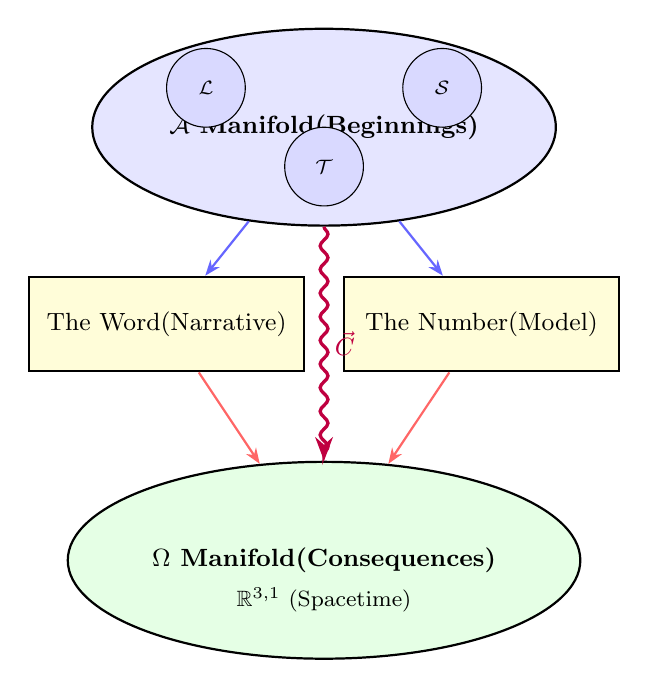
\begin{tikzpicture}[
    realm/.style={ellipse, minimum width=4cm, minimum height=2.5cm, 
                  text centered, draw=black, thick, font=\small\bfseries},
    interface/.style={rectangle, minimum width=3.5cm, minimum height=1.2cm,
                      text centered, draw=black, thick, fill=yellow!15, font=\small},
    component/.style={circle, minimum size=1cm, draw=black, fill=blue!15, font=\scriptsize},
    arrow/.style={-{Stealth[length=2mm]}, thick},
    label/.style={font=\footnotesize}]
    
    % Alpha realm (top)
    \node[realm, fill=blue!10] (alpha) at (0,6) {$\mathcal{A}$ Manifold\\(Beginnings)};
    \node[component] (love) at (-1.5,6.5) {$\mathcal{L}$};
    \node[component] (truth) at (0,5.5) {$\mathcal{T}$};
    \node[component] (meaning) at (1.5,6.5) {$\mathcal{S}$};
    
    % Psyche interface (middle)
    \node[interface] (word) at (-2,3.5) {The Word\\(Narrative)};
    \node[interface] (number) at (2,3.5) {The Number\\(Model)};
    
    % Omega realm (bottom)
    \node[realm, fill=green!10] (omega) at (0,0.5) {$\Omega$ Manifold\\(Consequences)};
    \node[label] at (0,0) {$\mathbb{R}^{3,1}$ (Spacetime)};
    
    % Connections
    \draw[arrow, blue!60] (alpha) -- (word);
    \draw[arrow, blue!60] (alpha) -- (number);
    \draw[arrow, red!60] (word) -- (omega);
    \draw[arrow, red!60] (number) -- (omega);
    
    % Christ-vector
    \draw[-{Stealth[length=3mm]}, very thick, purple, decorate, 
          decoration={snake, amplitude=0.5mm, segment length=3mm}] 
          (alpha) -- node[right, font=\small\bfseries, purple] {$\vec{C}$} (omega);
    
\end{tikzpicture}
\caption{The $\mathcal{A}\pi\text{-}\pi\Omega$ manifold structure showing the flow from abstract beginnings ($\mathcal{A}$) through linguistic interfaces ($\pi\text{-}\pi$) to physical consequences ($\Omega$). The Christ-vector $\vec{C}$ (purple) represents a direct geodesic path optimizing across all levels.}
\label{fig:manifold_structure}
\end{figure}

\begin{figure}[h!]
\centering
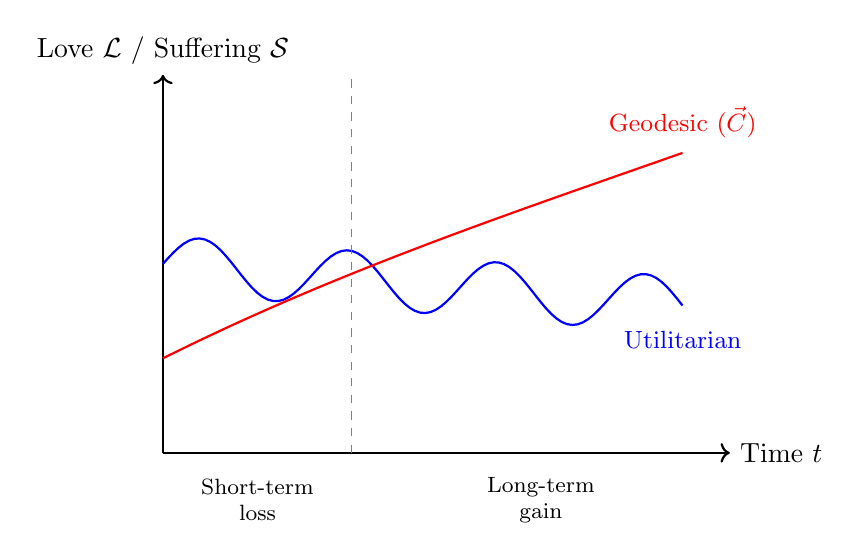
\begin{tikzpicture}[scale=1.2]
    % Axes
    \draw[->, thick] (0,0) -- (6,0) node[right] {Time $t$};
    \draw[->, thick] (0,0) -- (0,4) node[above] {Love $\mathcal{L}$ / Suffering $\mathcal{S}$};
    
    % Conventional path (oscillating, eventually declining)
    \draw[blue, thick, domain=0:5.5, samples=100] plot (\x, {2 + 0.3*sin(4*\x r) - 0.08*\x});
    \node[blue, font=\small] at (5.5, 1.2) {Utilitarian};
    
    % Geodesic path (initially lower, then rising steadily)
    \draw[red, thick, domain=0:5.5, samples=100] plot (\x, {1 + 0.5*\x - 0.03*\x*\x + 0.002*\x*\x*\x});
    \node[red, font=\small] at (5.5, 3.5) {Geodesic ($\vec{C}$)};
    
    % Annotations
    \draw[dashed, gray] (2,0) -- (2,4);
    \node[font=\footnotesize, align=center] at (1, -0.5) {Short-term\\loss};
    \node[font=\footnotesize, align=center] at (4, -0.5) {Long-term\\gain};
    
\end{tikzpicture}
\caption{Conceptual comparison of conventional utilitarian approaches versus the Christ-vector geodesic over generational time. The geodesic path may require initial sacrifice but optimizes long-term Love while minimizing cumulative Suffering.}
\label{fig:geodesic_comparison}
\end{figure}

% Extended trajectory comparison graphs for S.V.E. IV
% Insert this after the original Figure 3 in your document

\begin{figure}[h!]
\centering
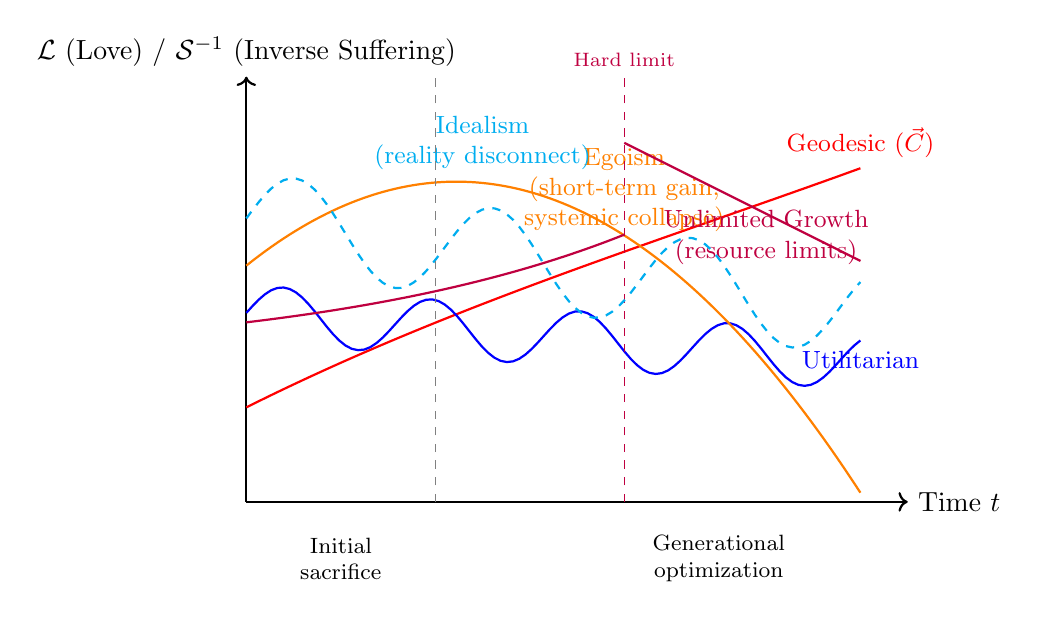
\begin{tikzpicture}[scale=1.2]
    % Axes
    \draw[->, thick] (0,0) -- (7,0) node[right] {Time $t$};
    \draw[->, thick] (0,0) -- (0,4.5) node[above] {$\mathcal{L}$ (Love) / $\mathcal{S}^{-1}$ (Inverse Suffering)};
    
    % Geodesic path (Christ-vector)
    \draw[red, thick, domain=0:6.5, samples=100] 
        plot (\x, {1 + 0.5*\x - 0.03*\x*\x + 0.002*\x*\x*\x});
    \node[red, font=\small] at (6.5, 3.8) {Geodesic ($\vec{C}$)};
    
    % Utilitarian path (oscillating, declining)
    \draw[blue, thick, domain=0:6.5, samples=100] 
        plot (\x, {2 + 0.3*sin(4*\x r) - 0.08*\x});
    \node[blue, font=\small] at (6.5, 1.5) {Utilitarian};
    
    % Egoism path (quick rise, sharp collapse)
    \draw[orange, thick, domain=0:6.5, samples=100] 
        plot (\x, {2.5 + 0.8*\x - 0.18*\x*\x});
    \node[orange, font=\small, align=center] at (4, 3.3) {Egoism\\(short-term gain,\\systemic collapse)};
    
    % Capitalism/Growth path (exponential rise then hard limit)
    \draw[purple, thick, domain=0:4, samples=50] 
        plot (\x, {1.5 + 0.4*exp(0.3*\x)});
    \draw[purple, thick, domain=4:6.5, samples=50] 
        plot (\x, {3.8 - 0.5*(\x-4)});
    \node[purple, font=\small, align=center] at (5.5, 2.8) {Unlimited Growth\\(resource limits)};
    \draw[dashed, purple] (4,0) -- (4,4.5) node[above, font=\scriptsize] {Hard limit};
    
    % Idealism path (disconnected from reality, unstable)
    \draw[cyan, thick, domain=0:6.5, samples=100, dashed] 
        plot (\x, {3 + 0.5*sin(3*\x r) - 0.15*\x});
    \node[cyan, font=\small, align=center] at (2.5, 3.8) {Idealism\\(reality disconnect)};
    
    % Annotations
    \draw[dashed, gray] (2,0) -- (2,4.5);
    \node[font=\footnotesize, align=center] at (1, -0.6) {Initial\\sacrifice};
    \node[font=\footnotesize, align=center] at (5, -0.6) {Generational\\optimization};
    
\end{tikzpicture}
\caption{Comparative trajectories of different ethical and economic paradigms over generational time. The geodesic path (red) requires initial sacrifice but achieves sustainable long-term optimization. Egoism (orange) produces quick gains but collapses systemically. Unlimited growth models (purple) hit hard resource constraints. Idealism (cyan, dashed) oscillates due to disconnection from physical reality. Only the Christ-vector geodesic maintains stable, increasing societal well-being across generations.}
\label{fig:extended_trajectories}
\end{figure}


\begin{figure}[h!]
\centering
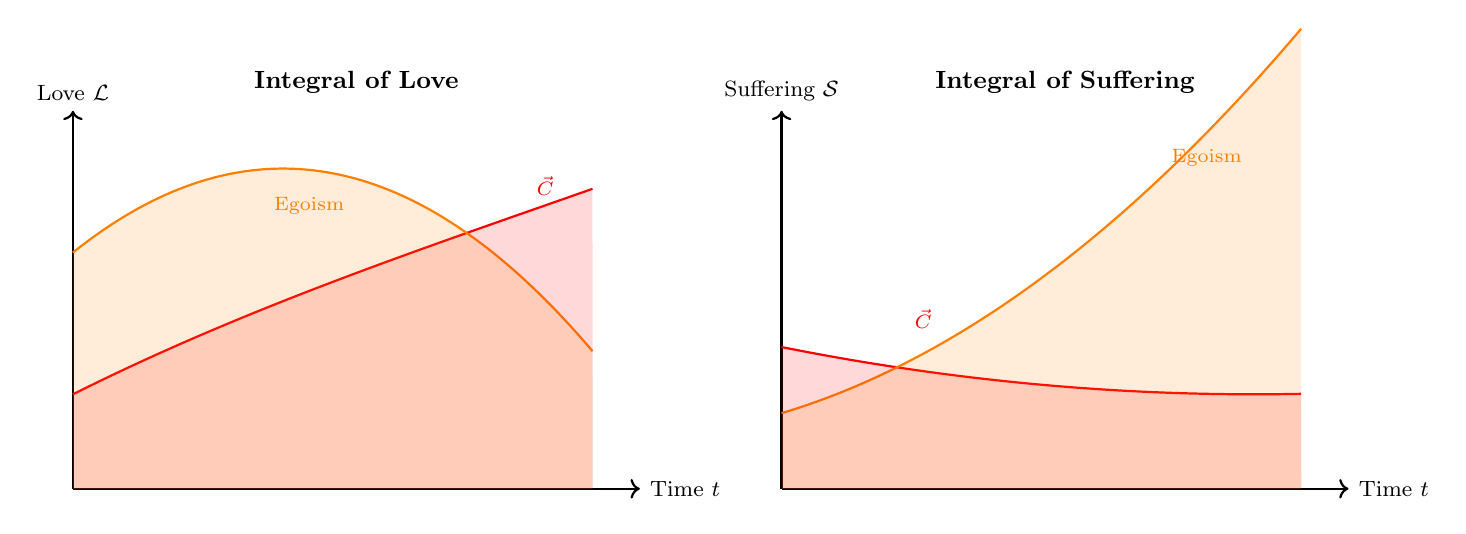
\begin{tikzpicture}[scale=1.2]
    % Two subplots side by side
    
    % LEFT: Love over time
    \begin{scope}[xshift=0cm]
    \draw[->, thick] (0,0) -- (6,0) node[right, font=\footnotesize] {Time $t$};
    \draw[->, thick] (0,0) -- (0,4) node[above, font=\footnotesize] {Love $\mathcal{L}$};
    \node[font=\small\bfseries] at (3, 4.3) {Integral of Love};
    
    % Christ-vector
    \draw[red, thick, domain=0:5.5, samples=100] 
        plot (\x, {1 + 0.5*\x - 0.03*\x*\x + 0.002*\x*\x*\x});
    
    % Egoism
    \draw[orange, thick, domain=0:5.5, samples=100] 
        plot (\x, {2.5 + 0.8*\x - 0.18*\x*\x});
    
    % Fill areas under curves
    \fill[red, opacity=0.15, domain=0:5.5, samples=100] 
        plot (\x, {1 + 0.5*\x - 0.03*\x*\x + 0.002*\x*\x*\x}) -- (5.5,0) -- (0,0);
    \fill[orange, opacity=0.15, domain=0:5.5, samples=100] 
        plot (\x, {max(0, 2.5 + 0.8*\x - 0.18*\x*\x)}) -- (5.5,0) -- (0,0);
    
    \node[red, font=\scriptsize] at (5, 3.2) {$\vec{C}$};
    \node[orange, font=\scriptsize] at (2.5, 3) {Egoism};
    \end{scope}
    
    % RIGHT: Suffering over time
    \begin{scope}[xshift=7.5cm]
    \draw[->, thick] (0,0) -- (6,0) node[right, font=\footnotesize] {Time $t$};
    \draw[->, thick] (0,0) -- (0,4) node[above, font=\footnotesize] {Suffering $\mathcal{S}$};
    \node[font=\small\bfseries] at (3, 4.3) {Integral of Suffering};
    
    % Christ-vector (low suffering)
    \draw[red, thick, domain=0:5.5, samples=100] 
        plot (\x, {1.5 - 0.2*\x + 0.02*\x*\x});
    
    % Egoism (high suffering)
    \draw[orange, thick, domain=0:5.5, samples=100] 
        plot (\x, {0.8 + 0.3*\x + 0.08*\x*\x});
    
    % Fill areas under curves
    \fill[red, opacity=0.15, domain=0:5.5, samples=100] 
        plot (\x, {1.5 - 0.2*\x + 0.02*\x*\x}) -- (5.5,0) -- (0,0);
    \fill[orange, opacity=0.15, domain=0:5.5, samples=100] 
        plot (\x, {0.8 + 0.3*\x + 0.08*\x*\x}) -- (5.5,0) -- (0,0);
    
    \node[red, font=\scriptsize] at (1.5, 1.8) {$\vec{C}$};
    \node[orange, font=\scriptsize] at (4.5, 3.5) {Egoism};
    \end{scope}
    
\end{tikzpicture}
\caption{Quantitative comparison of the geodesic optimization criterion (Equation~\ref{eq:geodesic}). Left panel shows accumulated Love over time; right panel shows accumulated Suffering. The shaded areas represent the integrals $\int \mathcal{L} \, dt$ and $\int \mathcal{S} \, dt$. The Christ-vector path maximizes the former while minimizing the latter, validating the geodesic hypothesis over generational timescales.}
\label{fig:integral_comparison}
\end{figure}

\begin{figure}[h!]
\centering
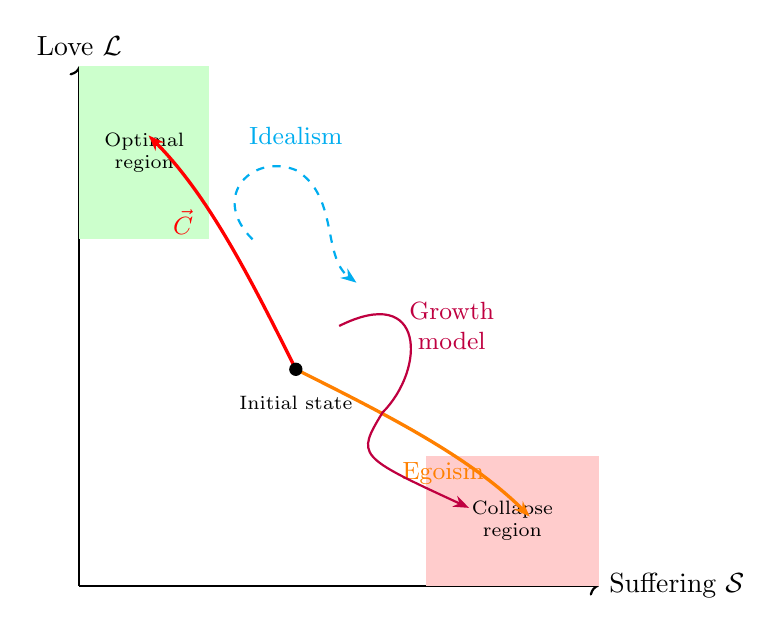
\begin{tikzpicture}[scale=1.1]
    % Phase space diagram: Love vs Suffering
    \draw[->, thick] (0,0) -- (6,0) node[right] {Suffering $\mathcal{S}$};
    \draw[->, thick] (0,0) -- (0,6) node[above] {Love $\mathcal{L}$};
    
    % Optimal region (high Love, low Suffering)
    \fill[green!20] (0,4) rectangle (1.5,6);
    \node[font=\scriptsize, align=center] at (0.75, 5) {Optimal\\region};
    
    % Collapse region (low Love, high Suffering)
    \fill[red!20] (4,0) rectangle (6,1.5);
    \node[font=\scriptsize, align=center] at (5, 0.75) {Collapse\\region};
    
    % Trajectories
    % Christ-vector: starts middle, moves to optimal
    \draw[-{Stealth[length=2mm]}, red, very thick] 
        (2.5, 2.5) .. controls (2, 3.5) and (1.5, 4.5) .. (0.8, 5.2);
    \node[red, font=\small] at (1.2, 4.2) {$\vec{C}$};
    
    % Egoism: starts middle, moves to collapse
    \draw[-{Stealth[length=2mm]}, orange, very thick] 
        (2.5, 2.5) .. controls (3.5, 2) and (4.5, 1.5) .. (5.2, 0.8);
    \node[orange, font=\small] at (4.2, 1.3) {Egoism};
    
    % Capitalism: circular then crash
    \draw[-{Stealth[length=2mm]}, purple, thick] 
        (3, 3) .. controls (4, 3.5) and (4, 2.5) .. (3.5, 2) .. controls (3.2, 1.5) .. (4.5, 0.9);
    \node[purple, font=\small, align=center] at (4.3, 3) {Growth\\model};
    
    % Idealism: oscillating, drifting
    \draw[-{Stealth[length=2mm]}, cyan, thick, dashed] 
        (2, 4) .. controls (1.5, 4.5) and (2, 5) .. (2.5, 4.8) .. controls (3, 4.5) and (2.8, 3.8) .. (3.2, 3.5);
    \node[cyan, font=\small] at (2.5, 5.2) {Idealism};
    
    % Starting point
    \filldraw[black] (2.5, 2.5) circle (2pt);
    \node[font=\scriptsize, below] at (2.5, 2.3) {Initial state};
    
\end{tikzpicture}
\caption{Phase space representation of ethical paradigms in the $(\mathcal{S}, \mathcal{L})$ plane. All systems start from a similar initial state, but follow different trajectories. The Christ-vector geodesic (red) navigates toward the optimal region of high Love and low Suffering. Egoistic strategies (orange) inevitably drift toward systemic collapse. Growth-focused capitalism (purple) exhibits cyclical behavior before resource-driven collapse. Idealistic approaches (cyan, dashed) oscillate without stable optimization due to disconnection from ground truth in $\Omega$.}
\label{fig:phase_space}
\end{figure}


% --- Appendix A: The Defiant Manifesto: The Scientific Protocol vFinal ---
\clearpage % Start on a new page

% Define colors if not already defined
\providecolor{headercolor}{RGB}{0, 51, 102}
\providecolor{accentcolor}{RGB}{0, 102, 204}


\section*{Appendix A. The Defiant Manifesto: The Scientific Protocol}
\addcontentsline{toc}{section}{Appendix A. The Defiant Manifesto: The Scientific Protocol}
\label{app:manifesto}

\vspace{1em}

\noindent\fcolorbox{accentcolor}{gray!5}{%
\begin{minipage}{\dimexpr\textwidth-2\fboxsep-2\fboxrule}
\textit{This appendix translates the moral courage of the original political manifesto into scientific clarity. Where politics defends through rhetoric, Systemic Verification Engineering (SVE) defends through reason. It embodies the \textbf{Socratic principle} by embracing critique as a catalyst for its own evolution. The text below specifies the philosophical antibodies of SVE—a self-healing discipline designed to thrive on challenge.}
\end{minipage}}

\vspace{1.5em}

\noindent\textbf{\textcolor{headercolor}{Core Premise.}} Their weapon is the appeal to captured authority. Our weapons are open methodology, logical rigor, radical transparency, and unwavering faith in the power of Truth. This document, like the SVE Protocol itself, is a living artifact; it will be publicly updated as new intellectual challenges emerge, turning every attack into evidence of its necessity and a catalyst for its reinforcement.

\vspace{1em}

% Scientific Lineage
\subsection*{\textcolor{headercolor}{Scientific Lineage}}
SVE stands in a lineage of transformative disciplines initially dismissed by the establishment: Darwinism (``pseudoscience''), Cybernetics (``ideology''), early Computer Science (``mere theory''). Each reshaped the paradigm it challenged. SVE follows this path: not a rejection of science, but its rehabilitation through verifiability, self-audit, and institutional design grounded in epistemic humility.

\vspace{1em}

% Attack 1
\subsection*{\textcolor{accentcolor}{Attack 1: ``This is Pseudoscience''}}

\paragraph{\textbf{Claim.}} SVE is non-rigorous; the ``Theorem on Disaster Prevention'' is a socio-probabilistic metaphor, not real mathematics; TRIZ is misapplied.

\paragraph{\textbf{Our Shield (Explanatory Power).}} We concede the Theorem is not pure mathematics; it is a \textbf{foundational axiom for an applied discipline}. Its validity stems from its predictive and explanatory power: modeling democracy as ``guessing the weight of an ox behind a closed door with expert labels'' accurately diagnoses real-world systemic failures (e.g., the Iraq War justification, the 2008 financial crisis, contradictory pandemic policies). SVE earns epistemic status by \textit{outperforming} existing institutional explanations in fidelity to observable outcomes.

\paragraph{\textbf{Our Counter (Public Intellectual Challenge).}} We invite critics to a live, recorded, long-form \textbf{epistemological boxing match}. They may deconstruct our methods under the SVE protocol itself; we will, in turn, apply the same protocol to audit the systemic failures their paradigms normalize. Let the public judge which approach better serves society: descriptive justifications from within a failing system, or an engineering blueprint designed to fix it.

\vspace{1em}

% Attack 2
\subsection*{\textcolor{accentcolor}{Attack 2: ``This is Ideology Disguised as Science''}}

\paragraph{\textbf{Claim.}} Christian ethics and concepts like ``multiplying love'' reveal inherent bias; the project is dogma masquerading as science.

\paragraph{\textbf{Our Shield (Architectural Separation of Fact and Value).}} SVE's three-stage architecture deliberately separates verifiable facts (\textit{``Caesar's realm''}) from value judgments (\textit{``God's realm''}). The protocol does not dictate morality; it secures a verified factual substrate upon which citizens can conduct informed deliberation. A scalpel in a Christian surgeon's hand remains a scalpel; function is defined by design and intent, not the wielder's faith.

\paragraph{\textbf{Our Counter (Demand for First Principles).}} We challenge critics to explicitly state the moral axioms underlying the status quo, which often tolerates dehumanizing logic (e.g., ``human resources,'' ``collateral damage''). Science devoid of declared ethics is not neutral; it is merely a tool available for hire by the highest bidder. We state our principles—rooted in the pursuit of truth and love—openly, and challenge others to do the same.

\vspace{1em}

% Attack 3
\subsection*{\textcolor{accentcolor}{Attack 3: ``This is Dangerous Science'' (The ``Ministry of Truth'' Gambit)}}

\paragraph{\textbf{Claim.}} A protocol capable of verifying truth could be weaponized by future tyrants to enforce a single narrative.

\paragraph{\textbf{Our Shield (Limited by Design \& Decentralized Trust).}} SVE is architected for \textbf{self-dissolution and decentralization}. The implementing institution (e.g., PFP party, SVE Foundation) is designed to create the tools, transfer copyright and control to a decentralized structure (the SVE DAO governed by a global community), and then disappear. It is the antithesis of a self-perpetuating ministry; it is a self-terminating catalyst for distributed verification.

\paragraph{\textbf{Our Counter (The True Danger is the Unverified Lie).}} The present and clear danger is not verified truth, but systemic, unchallengeable falsehood that paralyzes effective problem-solving and enables catastrophes. A democracy poisoned by lies is already a tyranny in disguise—a ``Ministry of Lies'' captured by hidden interests. SVE builds a shield for citizens against the tyranny that \textit{already exists}: the tyranny of the unaccountable lie.

\vspace{1em}

% Attack 4
\subsection*{\textcolor{accentcolor}{Attack 4: ``This is Politicized Science''}}

\paragraph{\textbf{Claim.}} Science is inherently contested and politicized (e.g., COVID-19, climate change); no objective protocol can arbitrate truth.

\paragraph{\textbf{Our Shield (Radical Honesty about Systemic Failure).}} We agree unequivocally: establishment science \textit{has been} deeply politicized and captured. This capture is not an argument against independent verification—it is the \textbf{primary justification} for it.

\paragraph{\textbf{Our Counter (The Protocol is the Cure, Not the Disease).}} SVE does not add another biased expert opinion to the fray. It installs a \textbf{meta-structure} that audits the experts themselves, separates factual claims from political spin, and publishes transparent, reproducible audit trails. We are not entering the political fight \textit{as} scientists fighting for a particular outcome; we are applying engineering principles to repair the fundamentally broken \textit{process} by which science informs public life.

\vspace{1em}

% Attack 5
\subsection*{\textcolor{accentcolor}{Attack 5: ``This is Too Complex for the People''}}

\paragraph{\textbf{Claim.}} Theorems, protocols, DAOs—this is too complex for ordinary citizens; inherently elitist.

\paragraph{\textbf{Our Shield (Distinguishing Complexity from Obfuscation).}} Modern life is complex (e.g., car engines, smartphones), but good design provides simple interfaces (steering wheels, touchscreens). The status quo often weaponizes complexity as \textbf{obfuscation} to prevent accountability. SVE distinguishes necessary internal complexity (the engineering under the hood) from deliberate external opacity.

\paragraph{\textbf{Our Counter (The Complexity Translator).}} The Socratic AI assistants and the three-stage architecture are explicitly designed to act as \textbf{complexity translators}. They distill intricate realities into: (1) Verifiable factual building blocks, (2) A clear spectrum of expert interpretations and value judgments, and (3) An understandable basis for civic choice. We do not demand citizens become engineers; we empower them with a reliable steering wheel for navigating complexity.

\vspace{1em}

% Attack 6
\subsection*{\textcolor{accentcolor}{Attack 6: ``This Will Stifle Innovation''}}

\paragraph{\textbf{Claim.}} Rigorous verification requirements will slow down scientific progress and punish creative, unconventional ideas.

\paragraph{\textbf{Our Shield (Correction, Not Punishment; Contextual Rigor).}} The protocol's 44-day grace period and emphasis on intellectual honesty foster a culture of learning from error, not fear of it. Bold hypotheses are encouraged; fabricated data is not. Furthermore, the level of required rigor is contextual: exploratory research faces a different standard than clinical trial data determining public health policy.

\paragraph{\textbf{Our Counter (Innovation Requires a Solid Foundation).}} True scientific progress is slowed far more by building upon fraudulent or irreproducible findings than by careful verification. Chasing phantom results based on bad data wastes decades and billions. SVE accelerates meaningful progress by ensuring each step rests on solid ground. Trust is the lubricant of innovation.

\vspace{1em}

% Attack 7
\subsection*{\textcolor{accentcolor}{Attack 7: ``This is Arrogant Science''}}

\paragraph{\textbf{Claim.}} Claiming to approximate objective truth is intellectual hubris, especially in light of postmodern critiques showing the social construction of knowledge.

\paragraph{\textbf{Our Shield (Epistemic Humility Architected In).}} SVE explicitly rejects claims of absolute truth. It produces \textit{Iterative Facts}—version-controlled, provisional, falsifiable conclusions, each carrying a fully documented, publicly auditable chain of reasoning and acknowledged limitations. The protocol's strength lies precisely in its \textbf{institutionalized admission of fallibility}. It aims for the most reliable approximation of truth currently possible, knowing it will be superseded.

\paragraph{\textbf{Our Counter (What Constitutes True Arrogance?).}} True arrogance lies in the current system: anonymous reviewers wielding unaccountable power, captured agencies declaring safety without independent scrutiny, media monopolies acting as arbiters of truth without transparent methodology. SVE proposes radical transparency where opacity now reigns, falsifiability against dogma, and public accountability replacing impunity. Is it arrogant to demand that claims affecting millions of lives be verifiable?

\vspace{1.5em}

% Closing Principle
\subsection*{\textcolor{headercolor}{Closing Principle: Reflexive Truth and Service}}

Every valid system must contain a mechanism to question and correct itself. SVE institutionalizes this reflex: the permanent, transparent audit of power, of science, and critically, \textit{of its own conclusions}. In this paradox lies its incorruptibility: by structurally embracing its own fallibility, it becomes resistant to dogma and capture.

The Protocol is not a fortress built to defend a final truth; it is a mirror designed to reflect reality more clearly, iteration by iteration. It does not seek to win the argument, but to keep the argument honest, tethered to facts and logic. Its ultimate aim is not intellectual victory, but service—service to the truth, and through truth, service to love and the flourishing of all.

\vspace{2em}

% Quotes section with better spacing
\begin{center}
\begin{minipage}{0.9\textwidth}
\hrule height 0.5pt
\vspace{1em}

\noindent\textit{``Judge not, that you be not judged.''} --- Matthew 7:1

\vspace{0.6em}
\noindent\textit{``I know that I know nothing.''} --- Socrates

\vspace{0.6em}
\noindent\textit{``The first principle is that you must not fool yourself—and you are the easiest person to fool.''} --- Richard Feynman

\vspace{0.6em}
\noindent\textit{``In a time of deceit, telling the truth is a revolutionary act.''} --- Often attributed to George Orwell

\vspace{1em}
\hrule height 0.5pt
\vspace{1em}

{\fontencoding{T2A}\selectfont
\noindent\textit{«Учітеся, брати мої,\\
Думайте, читайте,\\
І чужому научайтесь,\\
Й свого не цурайтесь...»}\\
--- Т. Шевченко («І мертвим, і живим, і ненарожденним...», 1845)

\vspace{0.8em}
\noindent\textit{«Скажи мне, американец, в чём сила? Разве в деньгах? [...] А я вот думаю, что сила — в правде. У кого правда — тот и сильней.»}\\
--- Д. Багров / Сергей Бодров-мл. (\href{https://youtu.be/fz6lGsgEGZ8}{«Брат 2»})
}

\vspace{1em}
\hrule height 0.5pt
\vspace{1em}

\noindent\textit{Father, guide us, Your children, on the path of truth; teach us to love—ourselves and our neighbors.}

\vspace{0.8em}
\noindent\textit{«I am the way, and the truth, and the life.»} --- John 14:6

\vspace{0.4em}
\noindent\textit{«You shall love your neighbor as yourself.»} --- Matthew 22:39

\vspace{1em}
\noindent\textit{Soli Deo gloria.} (Glory to God alone.)

\vspace{0.5em}
\hrule height 0.5pt
\end{minipage}
\end{center}

% --- END Appendix A ---

\end{document}